
\section{Eventos asociados a Todos los Disparos en el rango 2014-2020 }	\label{ALL_modulacion}
	

En este trabajo se busca comparar los parámetros obtenidos con los eventos de Todos los Disparos con los parámetros de la reconstrucción oficial. Para esto se realizó un análisis de la señal $S_{38}$ sin la corrección del clima, siguiendo un proceso similar a la sección \ref{sin_corregir_s38}.



\subsection{Distribución de los eventos en función de $\sin^2\theta$}

La separación de los eventos en rango de $\sin^2\theta$ para los datos del Disparo Estándar se realizó debido a que distribuye los eventos con energía por encima de $3\,$EeV de forma uniforme en cada rango. En la Fig\,\ref{fig:bin_eventos_sin_2_theta} se muestran las distribuciones que tiene los eventos del Disparo Estándar en distintos rangos de tiempo y los eventos de Todos los Disparos por encima de $3\,$EeV y $1\,$EeV respectivamente. Se toman estos límites porque los disparos alcanzan eficiencia completa a partir de estos valores de energía.  Se observa que para el Disparo Estándar los eventos varian $\sim 2.5\%$ con respecto a la media para los dos rangos de tiempo, en cambio los eventos por encima de $1\,$EeV para Todos los Disparos tienen una variación de $\sim 10\%$ con respecto a media.

\begin{figure}[H]
  \begin{small}
    \begin{center}
      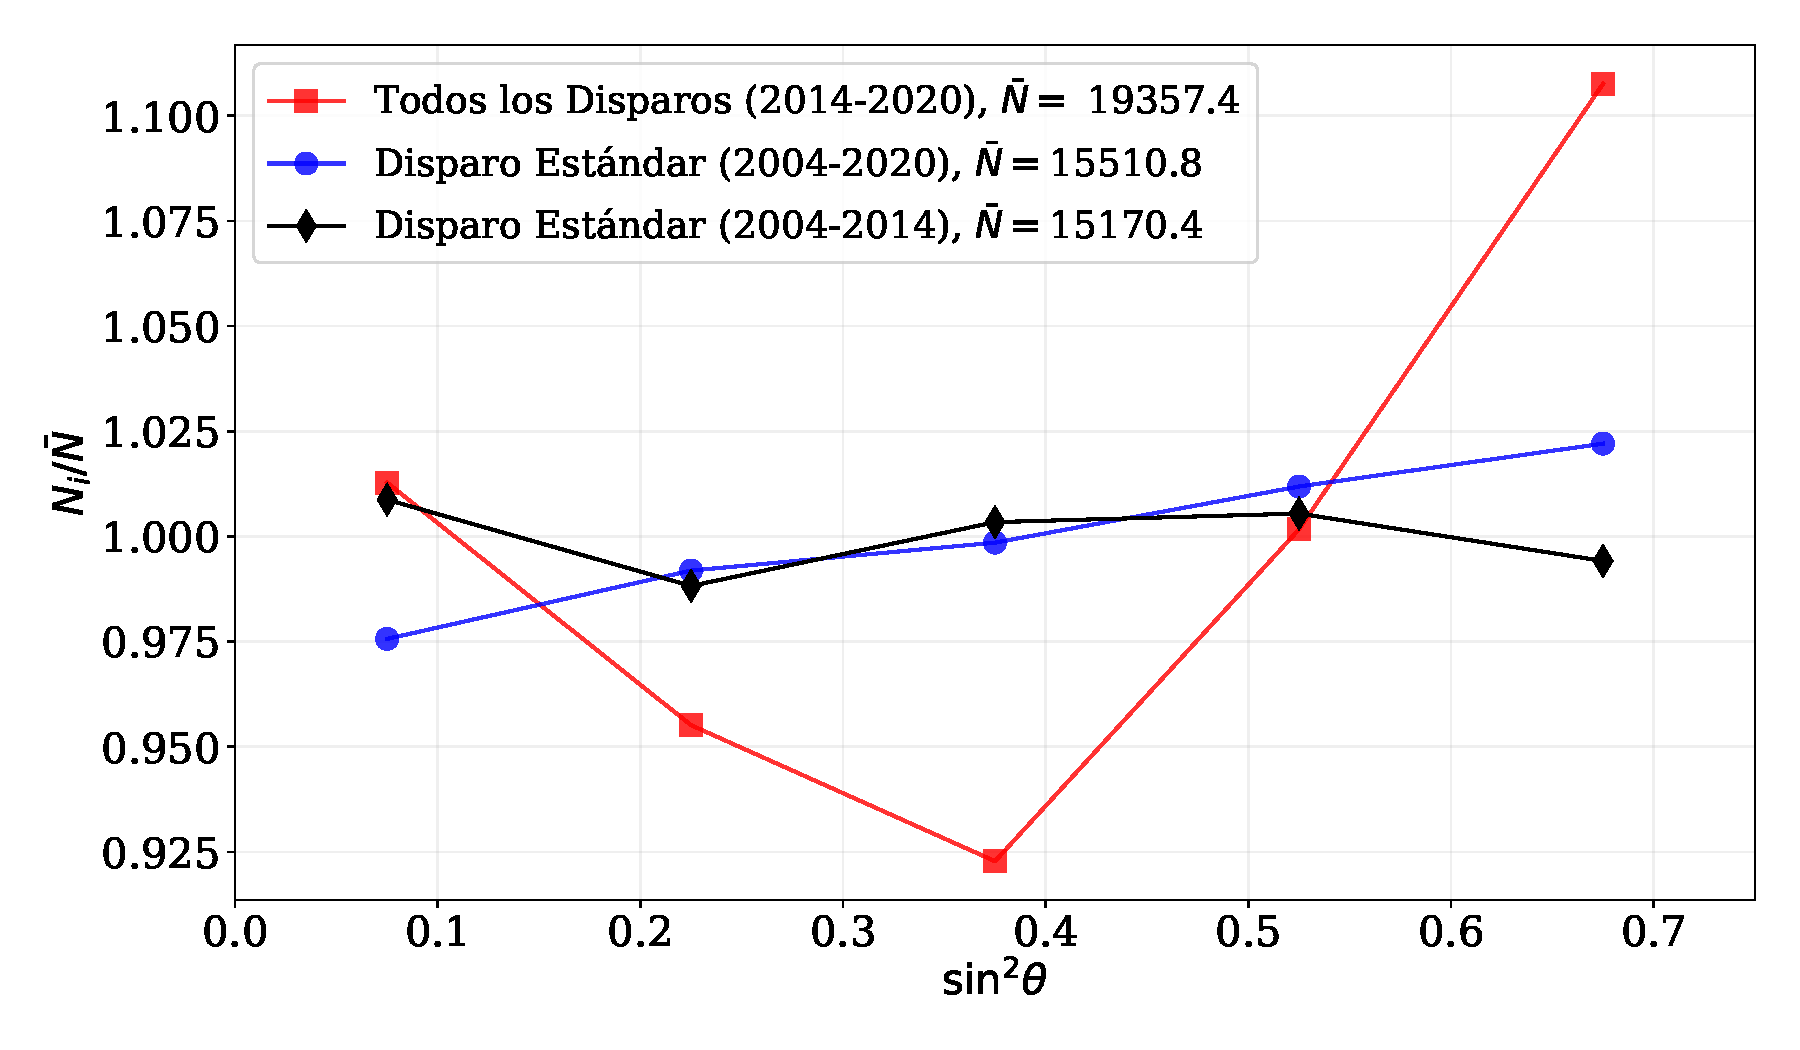
\includegraphics[width=0.8\textwidth]{bin_eventos_sin_2_theta.pdf}
    \end{center}
    \caption{Variación de eventos en cada rango de $\sin^2\theta$ respecto a la media para el Disparo Estándar y Todos los Disparos. }
    \label{fig:bin_eventos_sin_2_theta}
  \end{small}
\end{figure}
\subsection{Tasa de eventos de Todos los Disparos por encima de 1 EeV}

Los eventos de este conjunto de datos, la modulación espuria del clima está corregida con los parámetros obtenidos sobre el Disparo Estándar. Las tasas de eventos diario mostrados en la Fig.\,\ref{fig:rate_ALL}, por encima de 1 EeV y 2 EeV respectivamente, no muestran modulaciones importantes. En el caso de la tasa por encima de 1 EeV, se observa un remanente de modulación anual similar a los datos del ICRC 2019. 


\begin{figure}[H]
  \centering
  % \begin{subfigure}[b]{0.9\textwidth}
  % 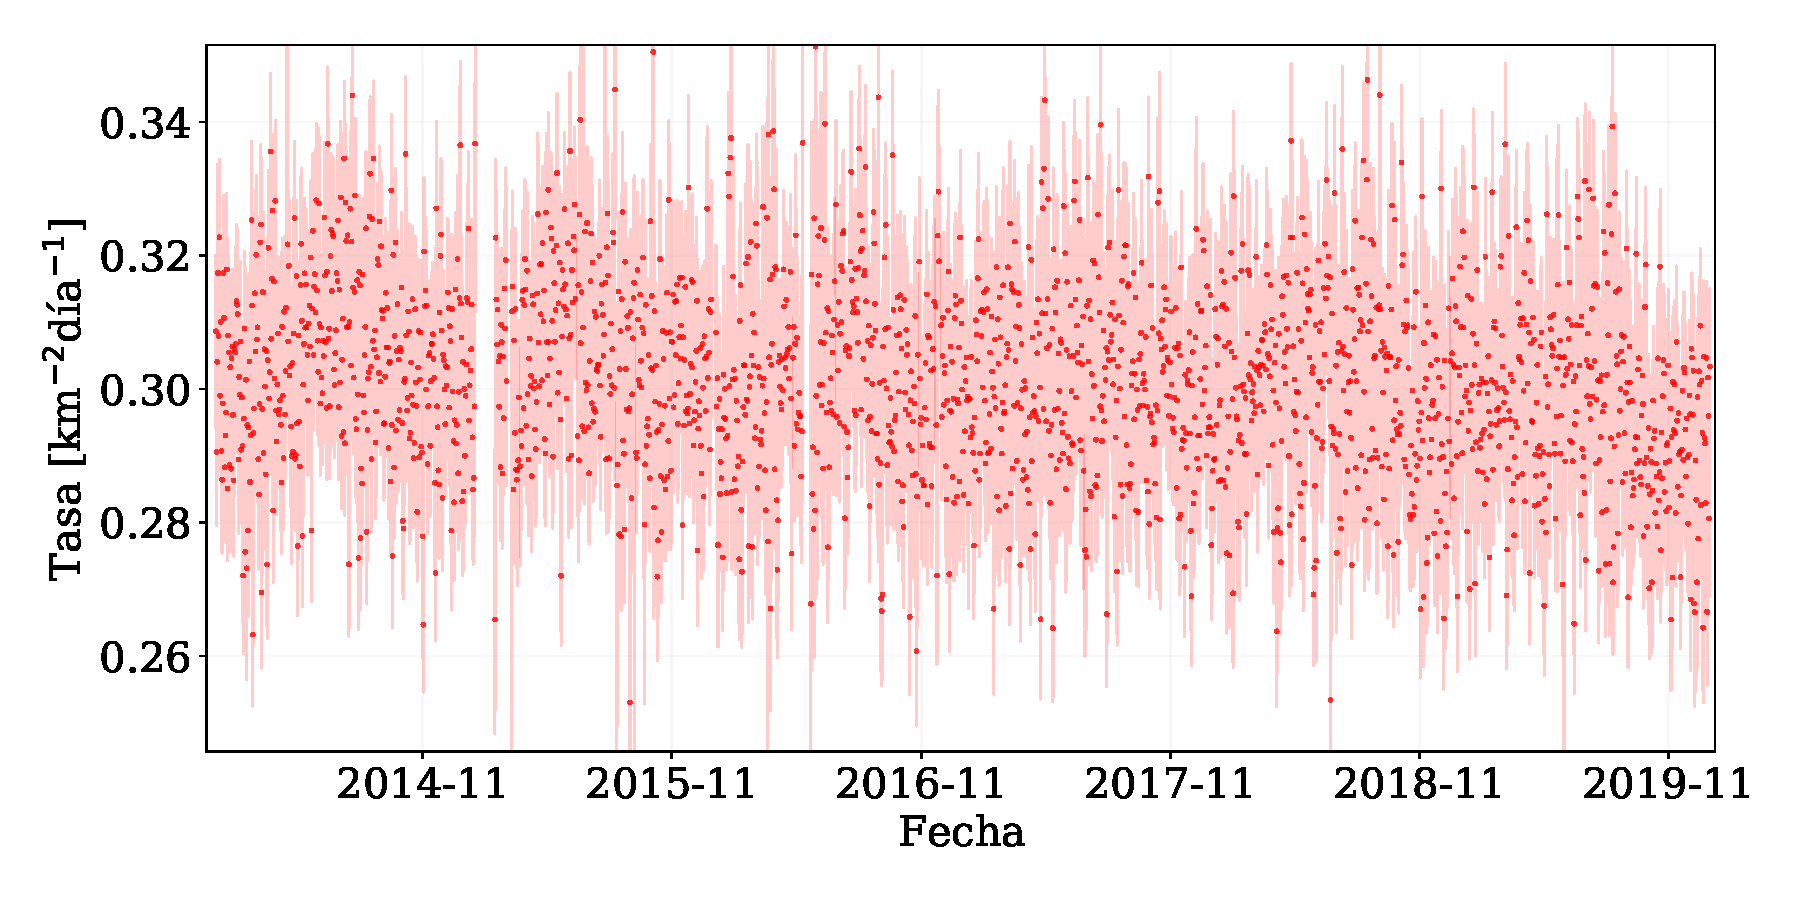
\includegraphics[width=\textwidth]{../04_Clima/Graphs/rate_dayly/AllTriggers_1EeV_rate_v3.pdf}
  % \caption{Energía mayor a $1\,$EeV}
  % \label{fig:rate_ALL_1}
  % \end{subfigure}\\
  % % \hspace{\fill}
  % \begin{subfigure}[b]{0.9\textwidth}
  % 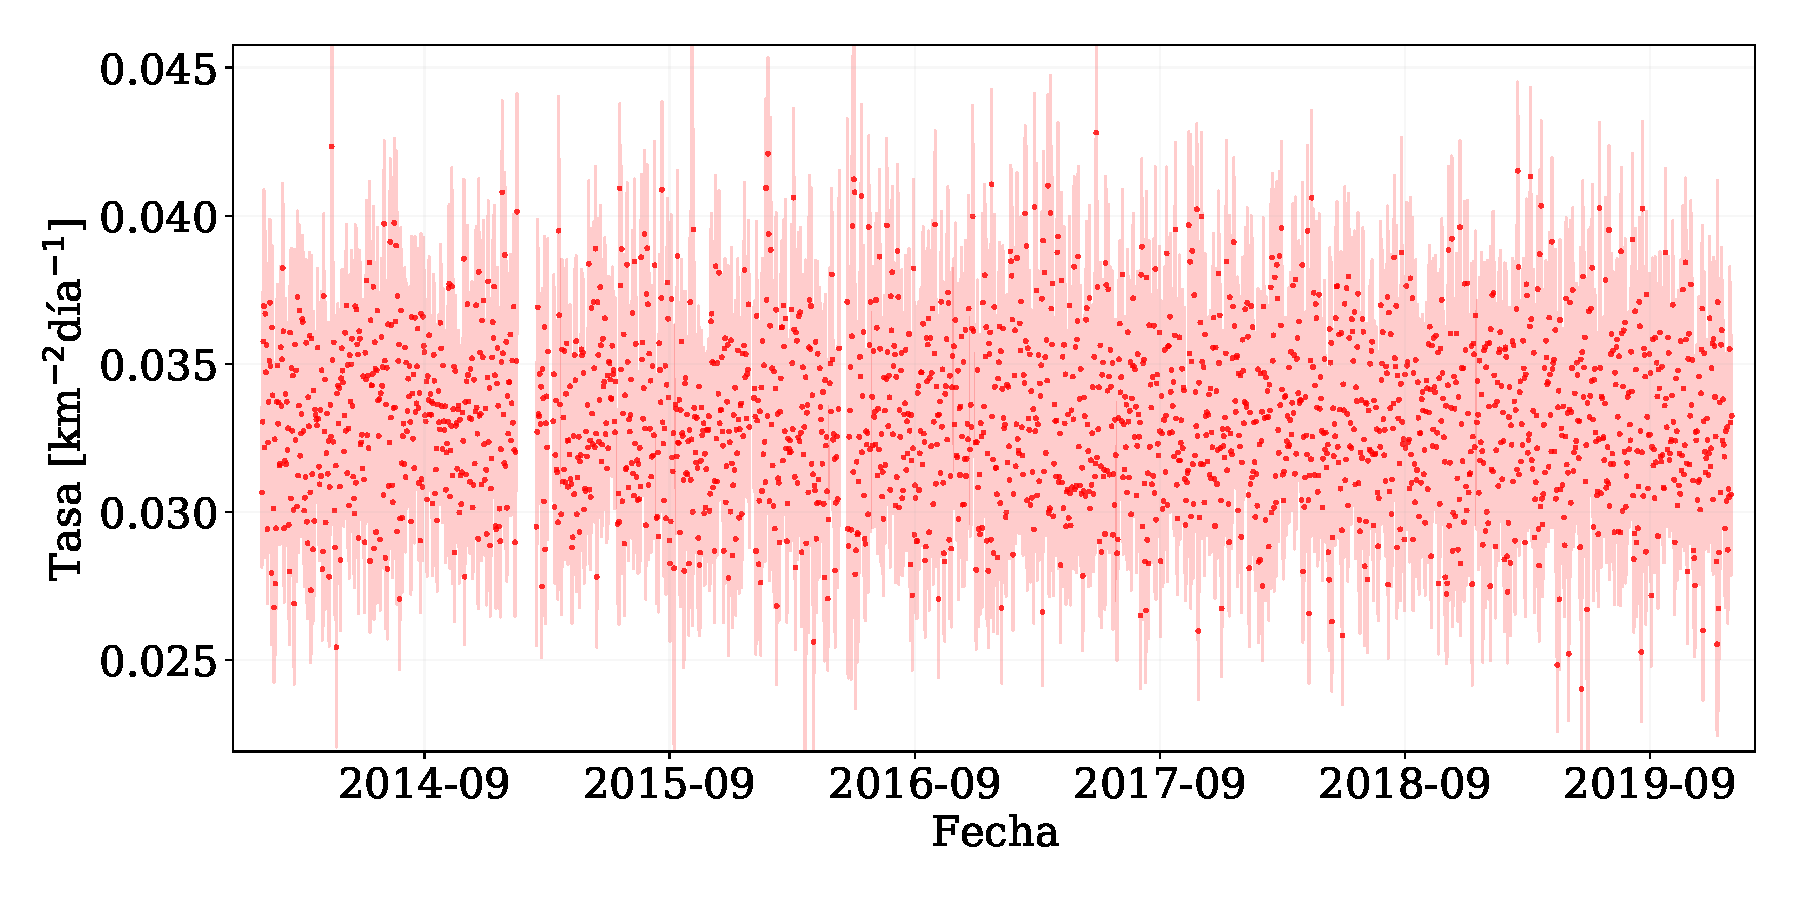
\includegraphics[width=\textwidth]{../04_Clima/Graphs/rate_dayly/AllTriggers_2EeV_rate.pdf}
  % \caption{ Energía mayor a $2\,$EeV}
  % \label{fig:rate_ALL_2}
  % \end{subfigure}%
  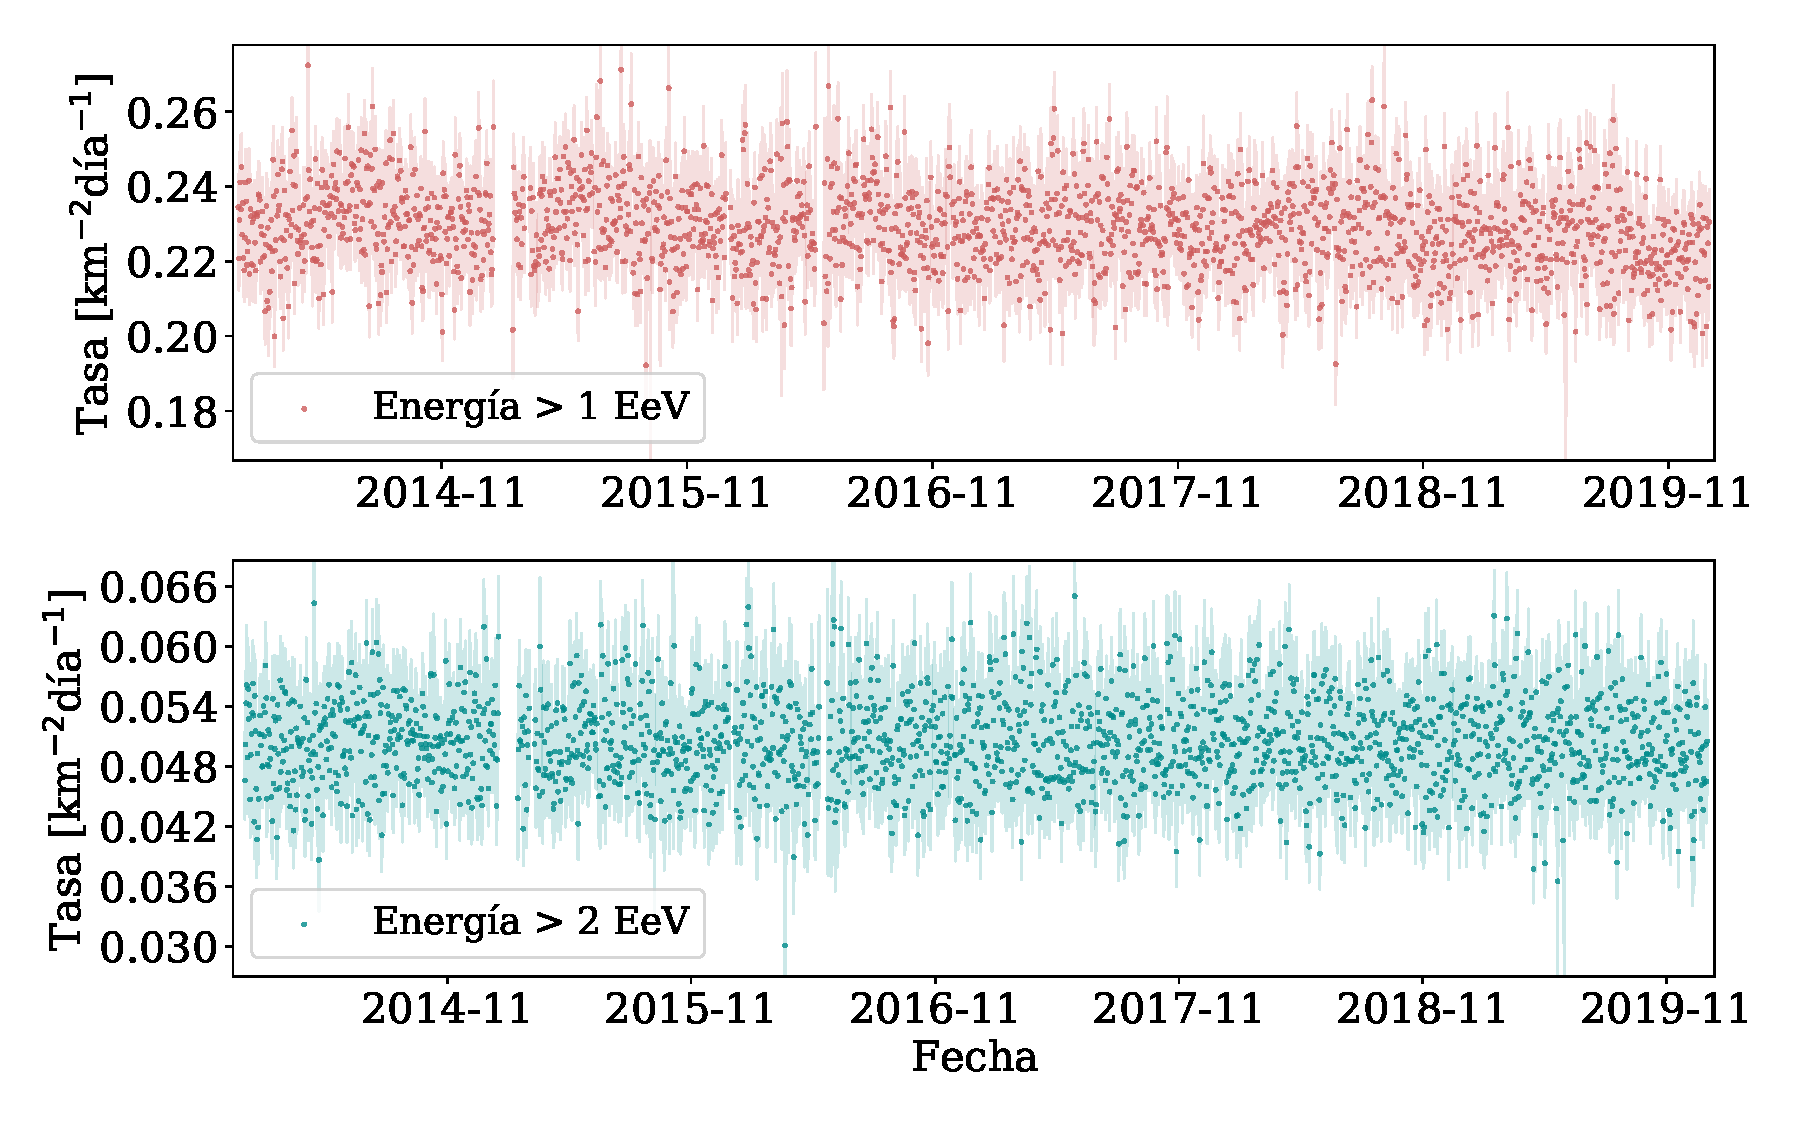
\includegraphics[width=\textwidth]{../04_Clima/Graphs/rate_dayly/AllTriggers_1EeV_2EeV_rate.pdf}
  \caption{Tasa de eventos promedio por cada día desde inicios del 2005 hasta inicios del 2020 de Todos los Disparos. Se muestran las tasas para dos cortes en energía, mayor a $1\,$EeV y mayor a $2\,$EeV}\label{fig:rate_ALL}
\end{figure}


\subsection{Parámetros del clima para Todos los Disparos usando $S_{38}$}


En esta sección, se trabajó con el conjunto de datos registrados por el arreglo principal con Todos los Disparos. La señal de $S(1000)$ de estos eventos fue corregida en la reconstrucción oficial de eventos por la modulación del clima por los parámetros obtenidos en \cite{aab2017impact}, por este motivo se trabajó con un corte en la señal de $S_{38}$ sin corregir por el clima. Las características de eventos obtenidos con el corte en la señal y otros filtros mencionados se resumen en la Tabla~\ref{tabla:caracteristicas_ALL}. 

\begin{table}[H]
  \centering
  \begin{tabular}{r|c|}
    \cline{2-2}
                & Todos los Disparos \\ \cline{2-2}
  Inicio:              & 01/01/2014\\ 
  Final:               & 01/01/2020       							\\ 
  Número de eventos:   & 1\,263\,015							\\ 
  Energía media:       & 1.76\,EeV       				\\  %  1.005\,EeV
  Corte en $S_{38}$:   & $>$5.36 VEM        				\\ 
  Corte en ángulo cenital:& $\theta < 60^o$ 				\\ \cline{2-2}
  \end{tabular}
\caption{Características del conjunto de datos de Todos los Disparos.} \label{tabla:caracteristicas_ALL}
\end{table}

Se realiza un ajuste de la tasa de eventos de Todos los Disparos y de esta manera se obtienen los coeficientes promediados por ángulo cenital. Los parámetros obtenidos se presentan y se comparan con los obtenidos sobre eventos del Disparo Estándar \cite{aab2017impact} en la Tabla \ref{tabla:parametros_ALL}. Los errores presentados son los errores obtenidos por el ajuste.  

\begin{table}[H]
  \centering
  \begin{tabular}{c|c|c}
  {Parámetro}                 & Todos los Disparos (2014-2020)& {2005-2015}    \cite{aab2017impact}              \\ \hline \hline
  $a_P$ [hPa$^{-1}$]          & $(-4.8 \pm 0.2)\times 10^{-3}$& $(-3.2 \pm 0.3)\times 10^{-3}$    \\ \hline
  $a_\rho$ [kg$^{-1}$m$^3$]   & $-1.54 \pm 0.04 $             & $-1.72 \pm 0.04$                  \\ \hline
  $b_\rho$ [kg$^{-1}$m$^3$]   & $-0.55 \pm 0.04$              & $-0.53 \pm 0.04$                  \\ \hline
  $\chi^2_\nu$                & $1.016$                       & $1.013$                           \\ 
  \end{tabular} 
  \caption{Ajustes obtenidos considerando todos los eventos con $\theta<60^o$ y energía mayor a $1\,$EeV del conjunto de Todos los disparos, comparados con los parámetros utilizados por la Colaboración.} \label{tabla:parametros_ALL}
\end{table}


La tasa de eventos media por día  medida y la tasa predicha según los parámetros del clima obtenidos se observan en la Fig.\ref{fig:rate_dayly_AllTriggers}. En la misma, la modulación anual y diaria del clima sobre los eventos es apreciable, a diferencia de las tasas de la Fig.\,\ref{fig:rate_ALL} donde  la energía de estos eventos están corregidos.  
\begin{figure}
\centering
  \begin{subfigure}[b]{0.9\textwidth}
  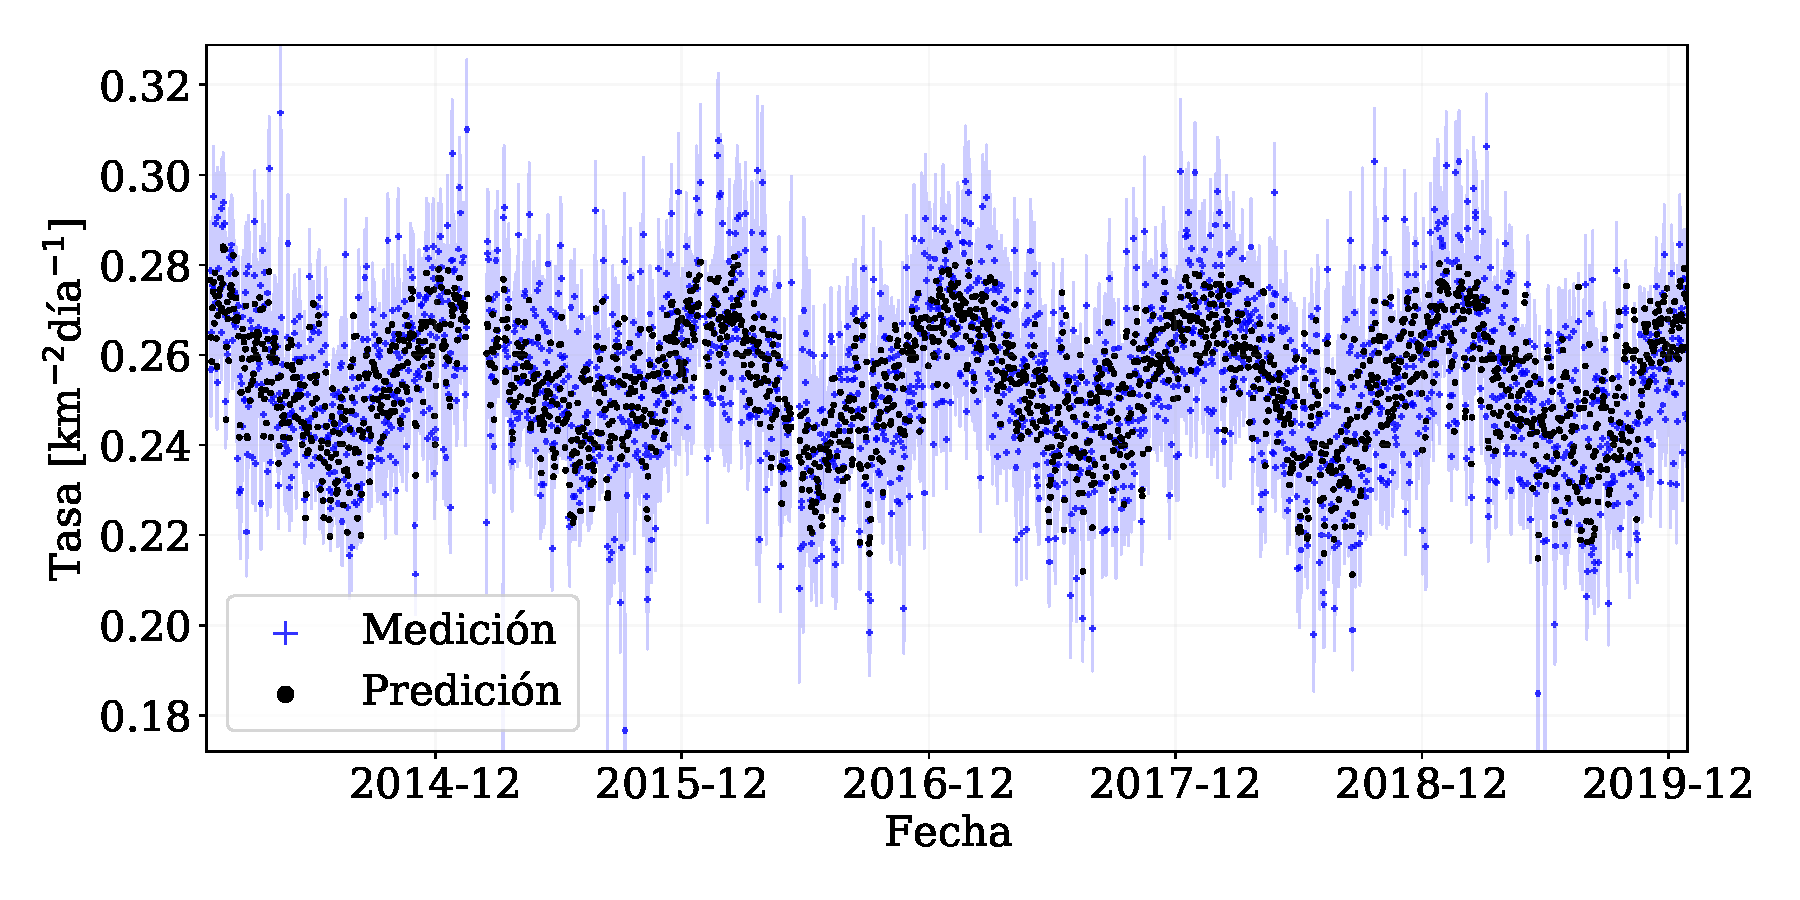
\includegraphics[width=\textwidth]{Graphs/rate_dayly/AllTriggers_S38_over_1EeV_rate_v3.pdf}
  \caption{Tasa eventos por día}\label{fig:rate_dayly_AllTriggers}
  \end{subfigure}\\
  \begin{subfigure}[b]{0.9\textwidth}
  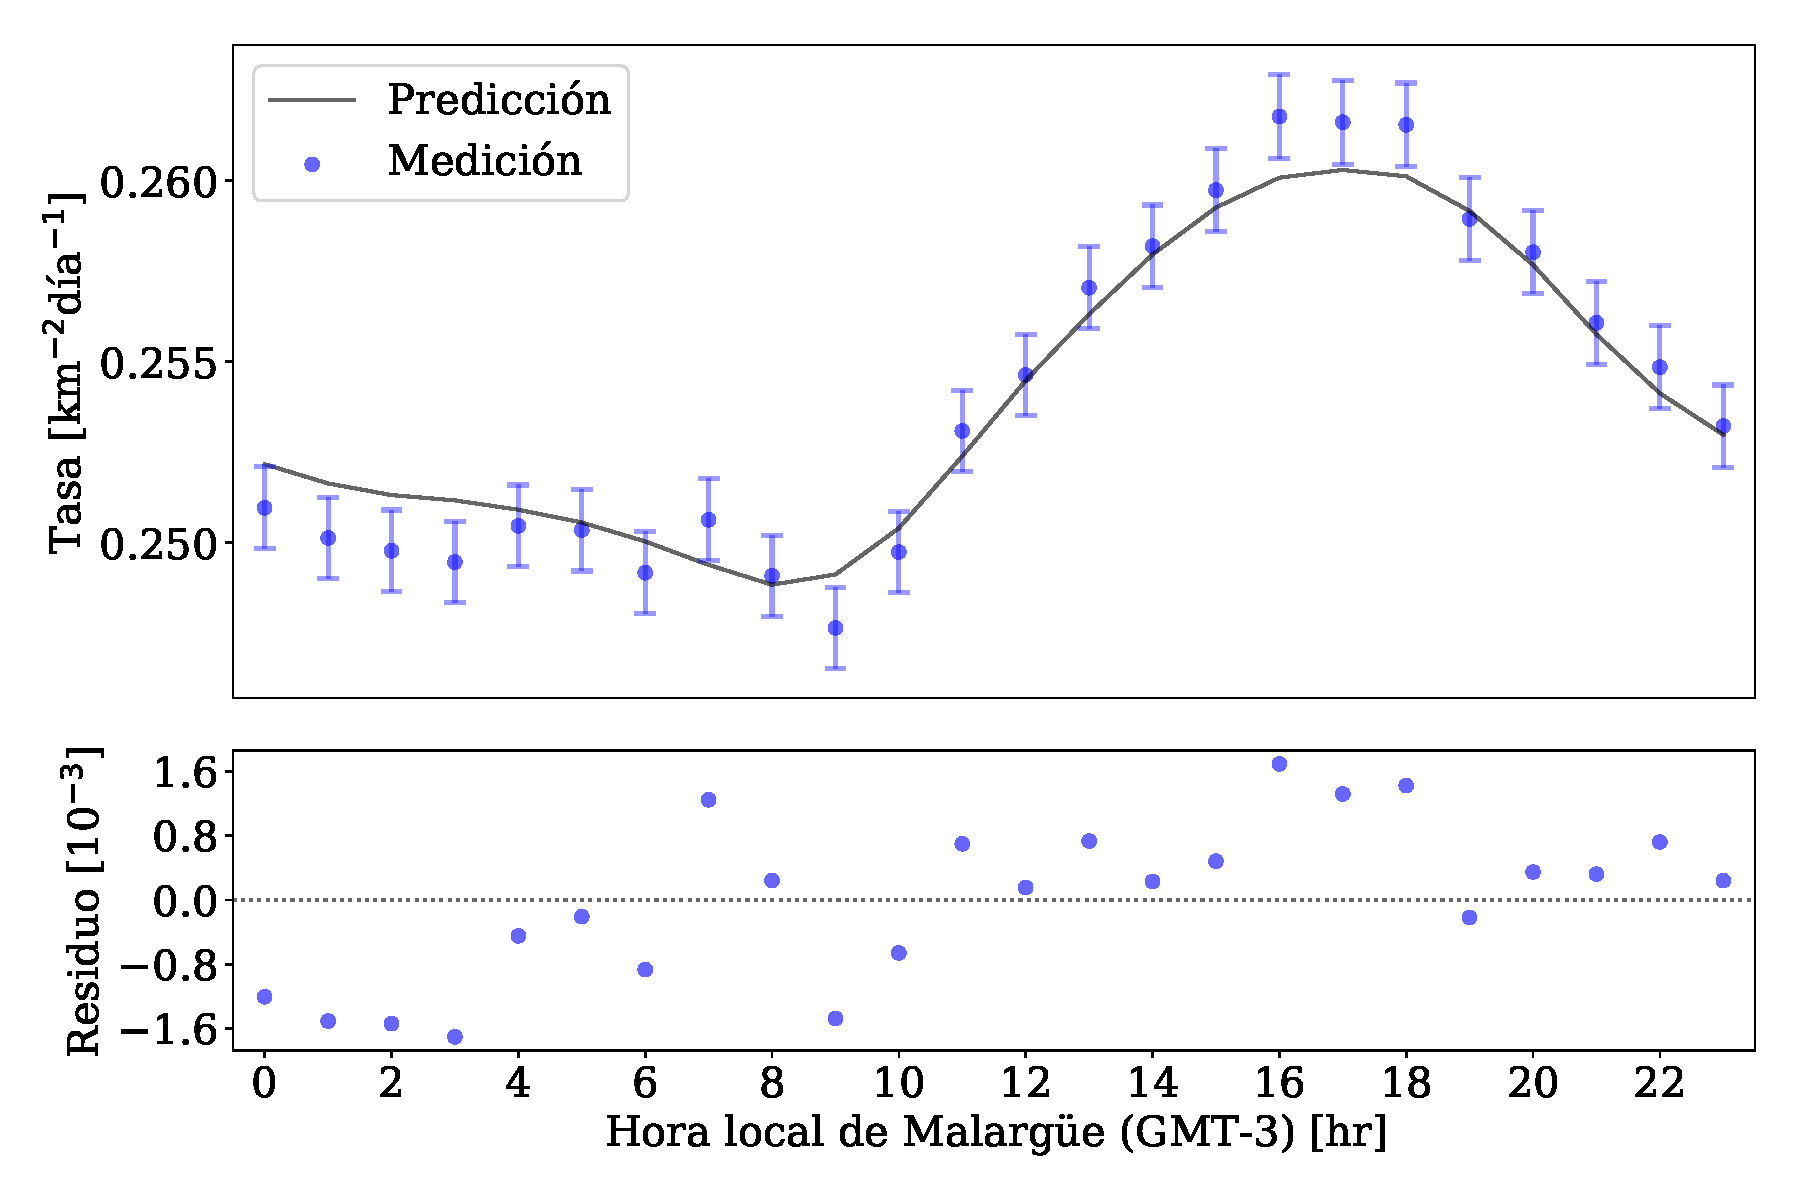
\includegraphics[width=\textwidth]{Graphs/rate_hour_of_the_day/AllTriggers_S38_over_1EeV_hour_of_the_day.pdf}
  \caption{Tasa de eventos promediada por hora del día }\label{fig:rate_hod_AllTriggers}
  \end{subfigure}
  \caption{Tasa de eventos por días comparadas con el ajuste entre los años 2014 hasta 2020. Estos eventos se registraron con Todos los Disparos  y tienen un valor de $S_{38}$ mayor a $5.36\,$VEM. En las tasas se observan la modulación anual y diaria del clima. La predicción es obtenida por los parámetros calculados en este trabajo.}\label{fig:rate__AllTriggers}
\end{figure}

Para poder verificar que los parámetros del clima en función de $\sin^2\theta$ obtenidos sobre el Disparo Estándar son válidos para Todos los Disparos, se calculó estos parámetros del último y se compararon con los utilizados por la Colaboración en la reconstrucción oficial. Estos resultados se observan en la Fig.\,\ref{fig:ALL-params} y los ajustes de la Ec.\,\ref{eq:cuadratica} se presentan en la Tabla~\ref{tabla:cuadratica_ALL}.   

\begin{figure}[H]
  \centering
  \begin{subfigure}[b]{0.75\textwidth}
  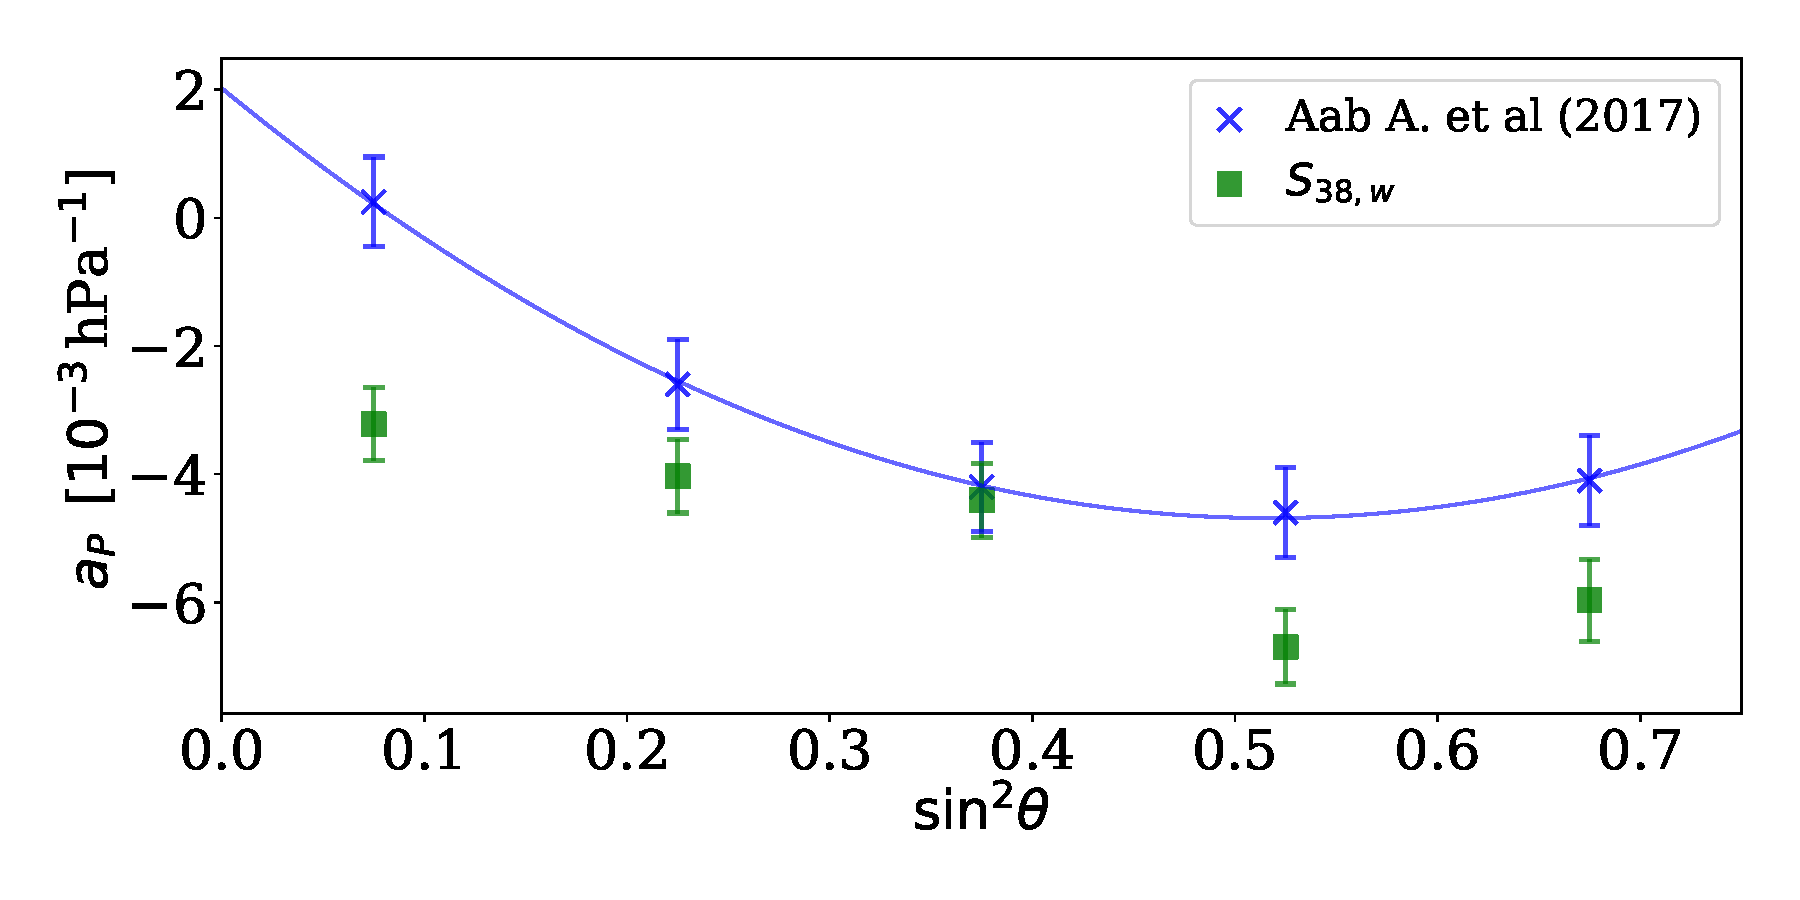
\includegraphics[width=\linewidth]{Graphs/params/ap_AllTriggers.pdf}
  \caption{Parámetro $a_P$ }
  \end{subfigure}\\
  \begin{subfigure}[b]{0.75\textwidth}
  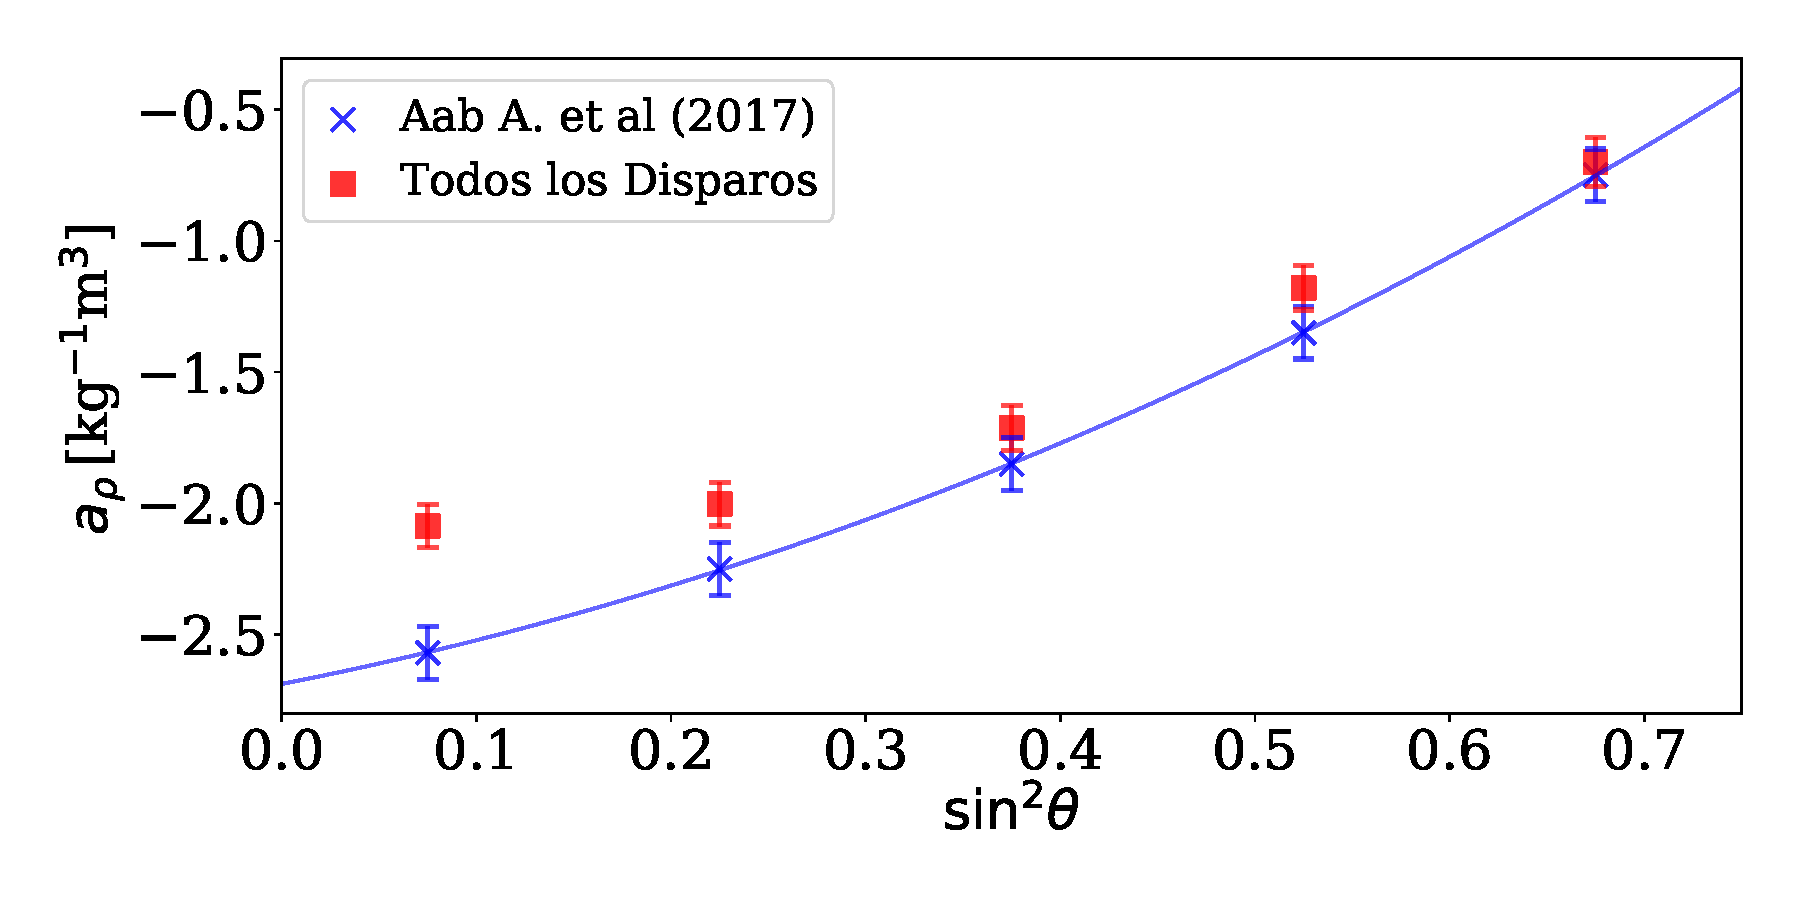
\includegraphics[width=\linewidth]{Graphs/params/arho_AllTriggers.pdf}
  \caption{Parámetro $a_{\rho}$ }
  \end{subfigure}\\
  \begin{subfigure}[b]{\textwidth}
  \centering
  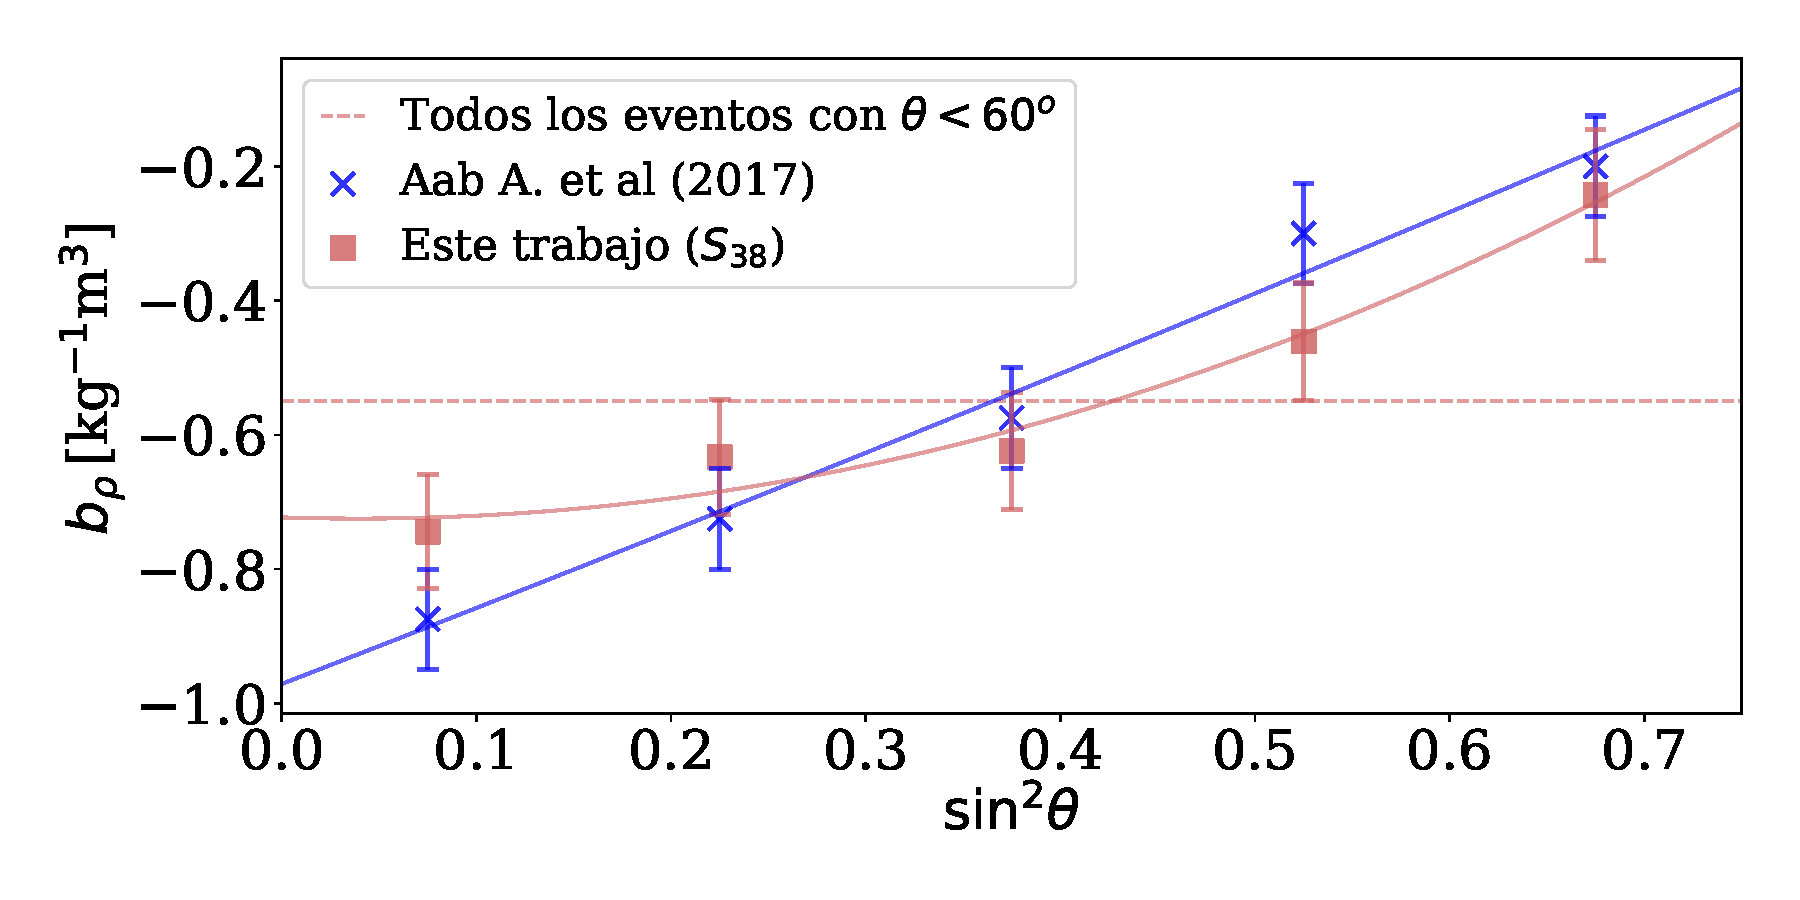
\includegraphics[width=0.75\linewidth]{Graphs/params/brho_AllTriggers.pdf}
  \caption{Parámetro  $b_\rho$   }
  \end{subfigure}
  \caption{Parámetros de la modulación del clima considerando los datos de Todos los Disparos, obtenido en el rango 2014-2020 . Los mismos se comparan con los coeficientes utilizados por la Colaboración \cite{aab2017impact}.}
  \label{fig:ALL-params}
\end{figure}

\begin{table}[H]
  \centering
  \begin{tabular}{l|l|l|l}
       Parámetros									& Coeficiente		& Todos los Disparos (2014-2020)	                  & \cite{aab2017impact}	\\ \hline \hline
   \multirow{3}{*}{$a_P$ [hPa$^{-1}$]}  			    &  $c_0$			& $( 2.5\pm 1.2)\times 10^{-3}$	& $( 2.1 \pm 0.9)\times 10^{-3} $	\\ \cline{2-4} %Done
                                                  &  $c_1$			& $(-8 \pm 8)\times 10^{-3}$	& $(-26.0 \pm 0.6 )\times 10^{-3}$	\\ \cline{2-4} 
                                                  &  $c_2$			& $( 0.0\pm 1.0)\times 10^{-3}$	& $( 26.0 \pm 0.7 )\times 10^{-3}$	\\ \hline \hline% 
  
   \multirow{3}{*}{$a_\rho$ [kg$^{-1}$m$^3$]}  	  &  $c_0$			& $-2.07   \pm 0.09$	            & $ -2.7  \pm 0.1  $\\ \cline{2-4} 
                                                  &  $c_1$			& $-0.0    \pm 0.5 $	            & $ 1.5   \pm 0.8  $\\ \cline{2-4} 
                                                  &  $c_2$			& $ 3.3    \pm 0.8 $	            & $ 2.2   \pm 1.0  $\\ \hline \hline%
  
  \multirow{3}{*}{$b_\rho$ [kg$^{-1}$m$^3$]} 		  &  $c_0$			& $-0.72   \pm 0.07$		            & $-1.0   \pm 0.1 $	\\ \cline{2-4} 
                                                  &  $c_1$			& $-0.0    \pm 0.4$		            & $ 1.2   \pm 0.8  $	\\ \cline{2-4} 
                                                  &  $c_2$			& $ 1.1    \pm 0.6$		            & $ 0.0   \pm 1.1  $	\\ 
  
  \end{tabular}	
  \caption{Tabla de los coeficientes obtenidos para Todos los Disparos, comparados con los parámetros de la reconstrucción de los eventos del Observatorio.} \label{tabla:cuadratica_ALL}
\end{table}


% \subsection{Pesos de los hexágonos en el rango 2014-2020}

% Para constatar que no exista ninguna anomalía en los pesos de los hexágonos, se realiza el cálculo de los mismos para tres frecuencias de referencia para el análisis de anisotropías.  Los pesos se muestran en la Fig.\,\ref{fig:wei_14_20}. El rango de tiempo en el que se calculan estas curvas es entre 1 de Enero del 2014 y el 1 de Enero del 2020.

% \begin{figure}[H]
% 	\centering
% 	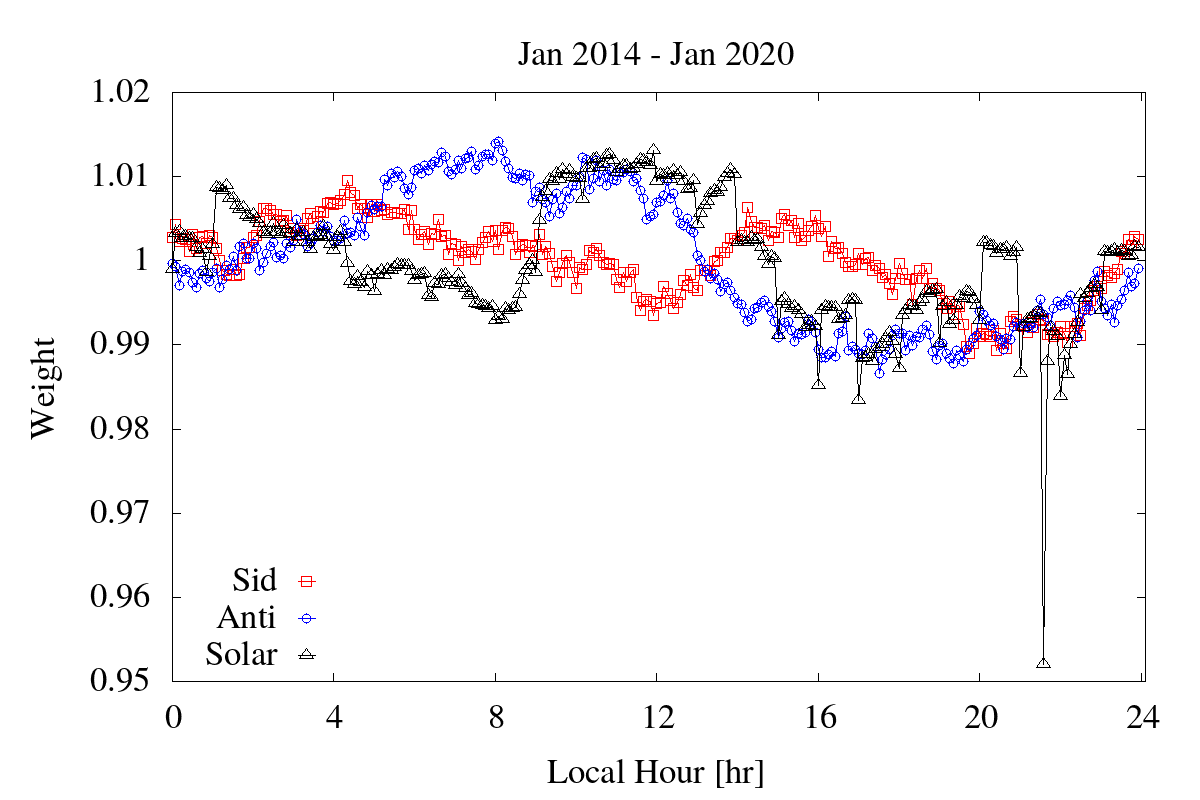
\includegraphics[width=0.5\textwidth]{weigth2014-2020_jan.png} 	
% 	\caption{Pesos de los hexágonos}
% 	\label{fig:wei_14_20}
% \end{figure}



      % Considerando el filtro con el S38 en el archivo 2020 y la energía en el 2017, quiero saber si obtengo parámetros  del clima comparables. Ya que el Main Array se corresponden los parámetros del 2015 y 2019, yo esperaría que con todos los triggers pase los mismo. Una diferencia importante entre ambos análisis es que los parámetros del 2020 contienen eventos hasta el 31/12/2019.
      
      % Los mismos se comparan con los ajustes obtenidos en \cite{aab2017impact}.

        % \begin{figure}[H]
        %   \centering
        %   \begin{subfigure}[b]{0.75\textwidth}
        %   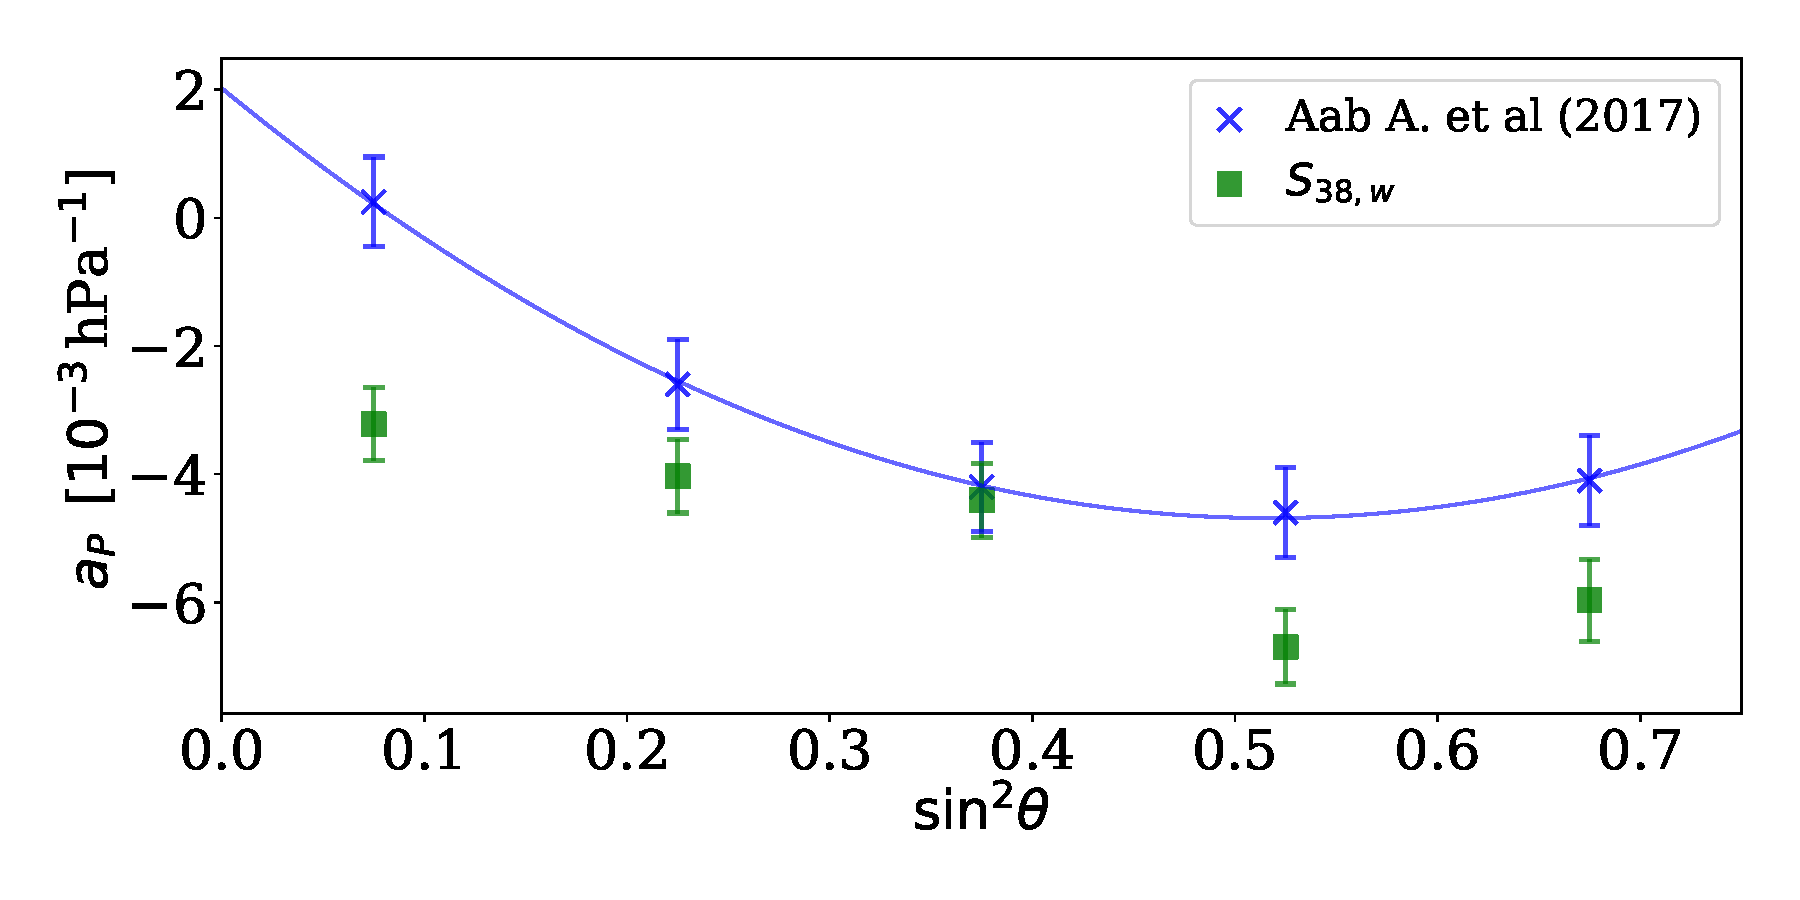
\includegraphics[width=\linewidth]{Graphs/params/ap_AllTriggers.pdf}
        %   \caption{Parámetro $a_P$ }
        %   \end{subfigure}\\
        %   \begin{subfigure}[b]{0.75\textwidth}
        %   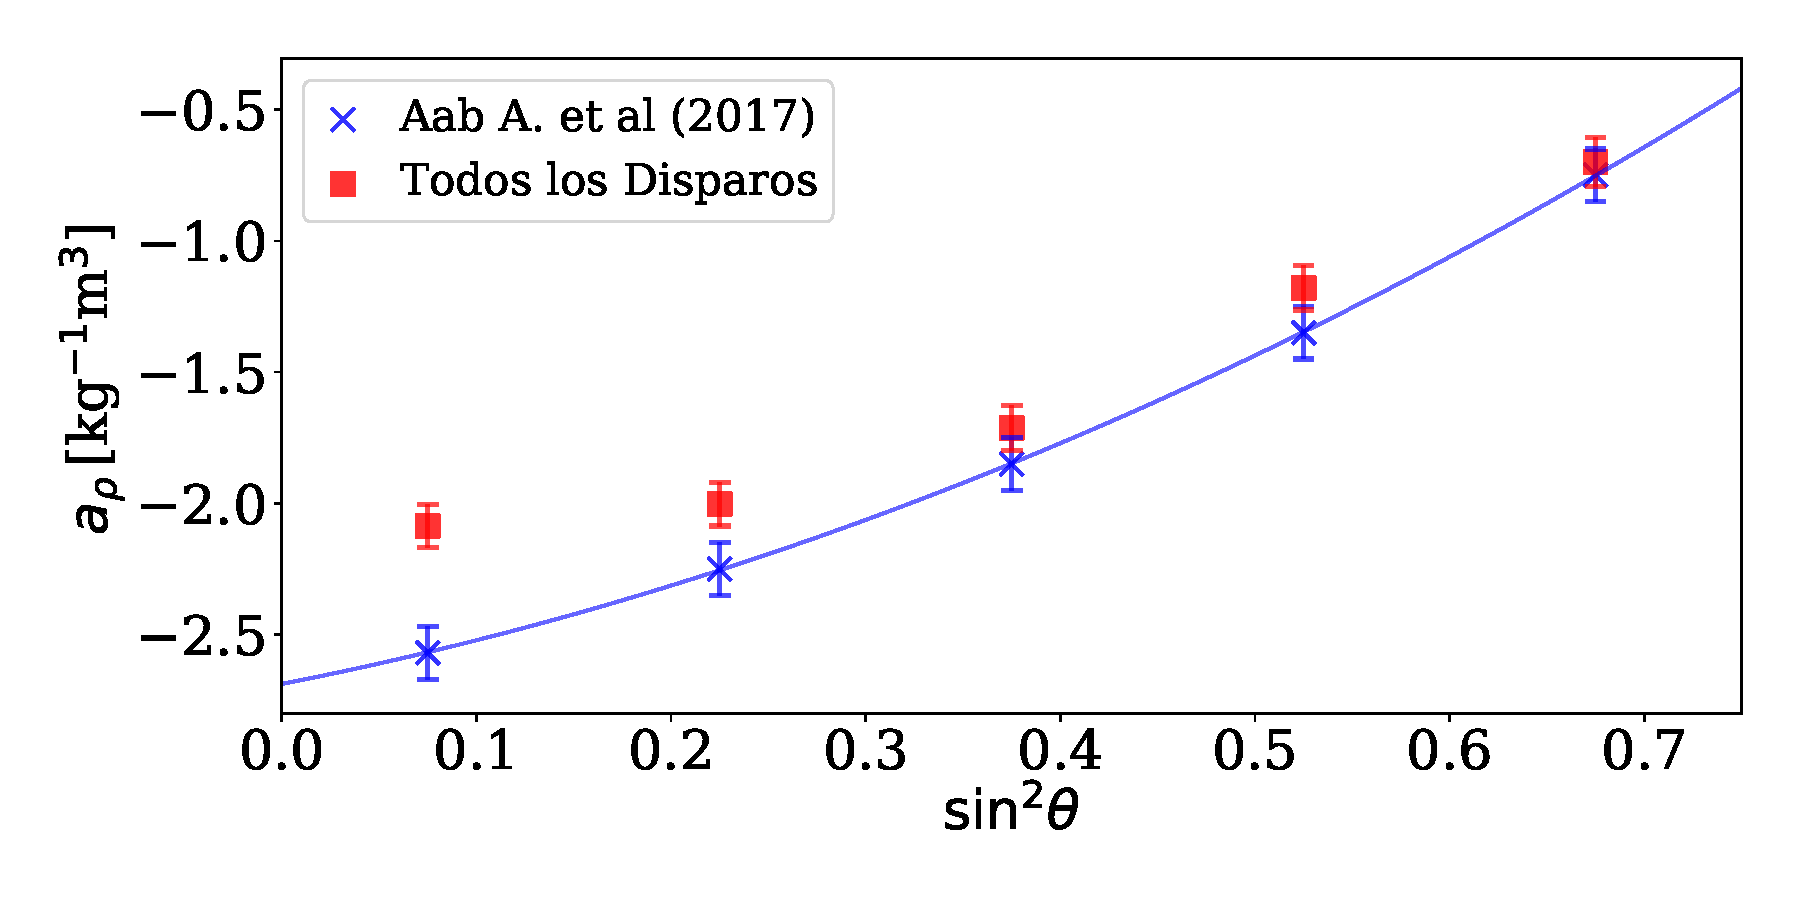
\includegraphics[width=\linewidth]{Graphs/params/arho_AllTriggers.pdf}
        %   \caption{Parámetro $a_{\rho}$ }
        %   \end{subfigure}\\
        %   \begin{subfigure}[b]{\textwidth}
        %   \centering
        %   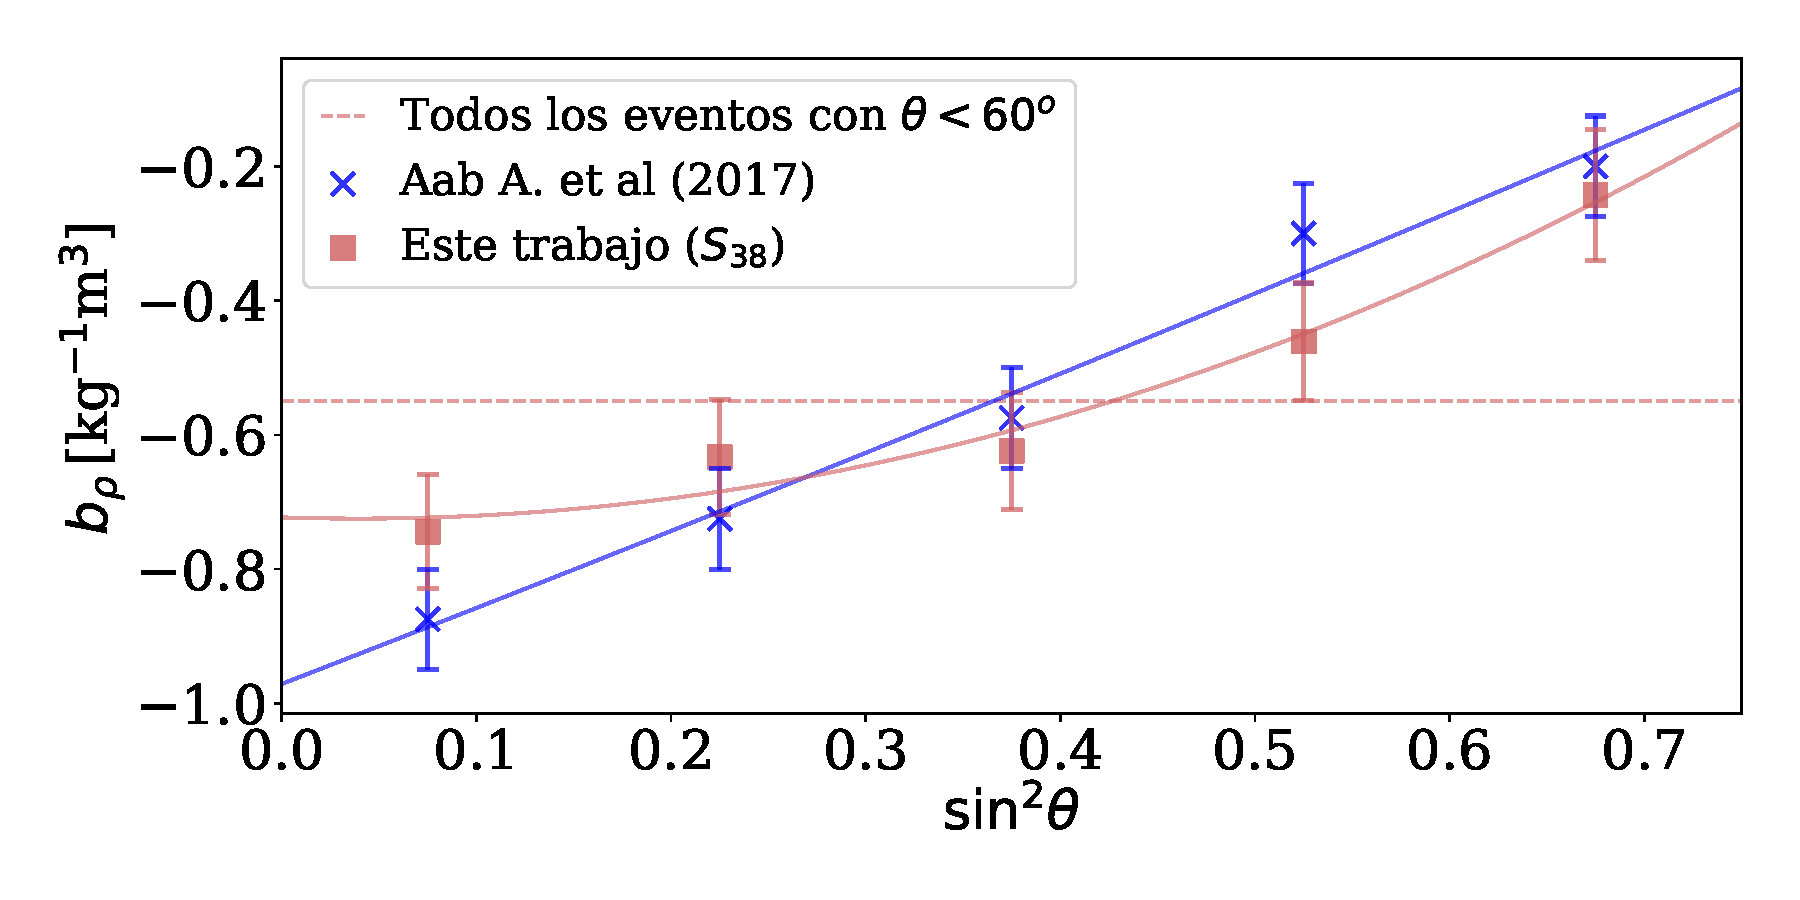
\includegraphics[width=0.75\linewidth]{Graphs/params/brho_AllTriggers.pdf}
        %   \caption{Parámetro  $b_\rho$   }
        %   \end{subfigure}
        %   \caption{Parámetros de la modulación del clima considerando los datos para Todos los Disparos del archivo 2017 y 2020. Los mismos se comparan con los coeficientes utilizados por la Colaboración.}
        % \end{figure}

%       ???????????Se ve que estos parámetros no son comparables. 
